% Glava dokumenta
\documentclass{beamer}
\usepackage[slovene]{babel}
\usepackage[utf8]{inputenc}
\usepackage{lmodern}
\usepackage[T1]{fontenc}
\usepackage{amssymb}
\usepackage{amsmath}
\usepackage{mathrsfs}
\usepackage{graphicx}
\usepackage{import}
\graphicspath{ {./slike/} }

\usepackage{pgf,tikz,pgfplots}
\usetikzlibrary{arrows}
\usepackage{lmodern}                            % to get rid of font warnings
\renewcommand\textbullet{\ensuremath{\bullet}}  % to get rid of font warnings

\usetheme{Warsaw} % izbira nastavitev oblike in barv strani
\beamertemplatenavigationsymbolsempty
%definicije izrekov----------
\newtheorem{izrek}{Izrek}
\newtheorem{df}{Definicija}
%Information to be included in the title page:
\title{Izrek o invarianci odprtih množic}
\author[Tom Gornik]{Avtor: Tom Gornik\\ \footnotesize Mentor: izr. prof. dr. Jaka Smrekar}
\institute{Fakulteta za matematiko in fiziko}
\date{\today}

\begin{document}
% Vsaka stran (prosojnica) je v okolju frame

\frame{\titlepage}

\begin{frame}

\frametitle{Zakaj izrek o invarianci odprtih množic?}

% Vsebina prosojnice 1
\begin{itemize}
\item Izgleda enostavno
\item Presenetljivo težko dokazati

\end{itemize}



\end{frame}

\begin{frame}

\frametitle{Izrek o invarianco odprtih množic}
% Vsebina prosojnice 2
\begin{overprint}
\onslide<1> \hfill\hyperlinkframestartnext{\beamerskipbutton{Skip Proof}}
\onslide<2>
\begin{proof}
Tukaj pa je dokaz, ki bi ga lahko preskočili \ldots.
\end{proof}
\end{overprint}

\end{frame}

\begin{frame}
\frametitle{Izrek o invarianci odprtih množic}
\framesubtitle{Podnaslov}
% Vsebina prosojnice 3
\begin{figure}[h!]
	\centering
	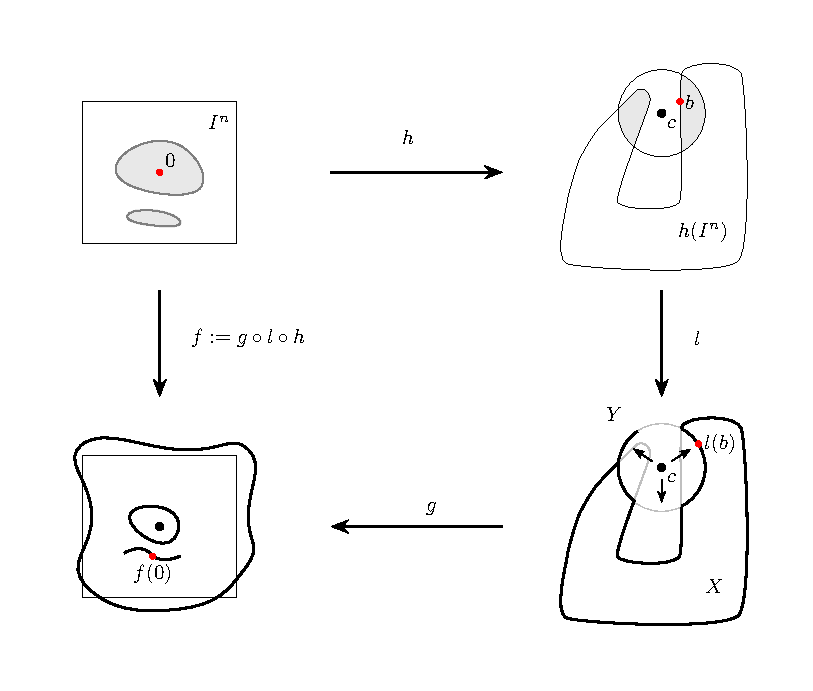
\includegraphics[scale=0.7]{glavna_slika.pdf}%
	\caption{Skica dokaza izreka.}
\end{figure}
\end{frame}

\begin{frame}
\frametitle{Izrek o invarianci odprtih množic}
\begin{block}{Izrek o invarianco odprtih množic}
Naj bo $U \subset \R^n$ odprta podmnožica evklidskega prostora $\R^n$ in naj bo $h : U \rightarrow \R^n$ zvezna injektivna preslikava.
Potem je tudi slika $h(U)$ odprta množica v $\R^n$.
\end{block}
\end{frame}


\end{document}

